% importa variabili globali
% definizione variabili globali
\def\GRUPPO {\textit{DazzleWorks}}

\def\PROGETTO {\textbf{Premi}}

\def\COMMITTENTE {Prof. Vardanega Tullio, \\ & Dr. Cardin Riccardo}

\def\EMAIL {dazzleworksgroup@gmail.com}

\def\LOGO {../../template/img/logo.png}

\def\INTESTAZIONE {../../template/img/intestazione.png}
\def\PIEDIPAGINA {../../template/img/piedipagina.png}

\def\G {{\small $_G$}}



% definizione variabili locali
\def\DOCUMENTO{Definizione di Prodotto}
\def\VERSIONE{1.0.0}

\def\DESCRIZIONE{Documento che definisce in dettaglio l'architettura del prodotto \PROGETTO.}

\def\REDATTORE {Burlin Valerio \\ & Carraro Nicola \\ & Crespan Emanuele \\ & Ros Fabio}
\def\VERIFICATORE {Agostinetto Matteo}
\def\RESPONSABILE {Suierica Bogdan}

\def\USO {Esterno}

\def\DISTRIBUZIONE {\GRUPPO{}\\ & \COMMITTENTE{}\\ & \PROPONENTE{}\\}

\def\DESCRIZIONE {Documento che definisce in dettaglio l'architettura del prodotto \PROGETTO.}


% abilita (true) / disabilita (false) indice, lista tabelle, lista figure
\def\INDICE	{true}
\def\TABELLE {true}
\def\FIGURE {true}


% importa struttura
\documentclass[a4paper]{article}

% ----- definizioni -----
\def\TITLE		{\mbox{\GRUPPO}}
\def\SUBTITLE	{\SIGLA, \PROGETTO}


% ----- nuovi comandi -----
% fornisce il caption per riferirsi ad una particolare sezione
\newcommand{\numref}[1]{\textsf{\textsl{``\nameref{#1}'' (\ref{#1})}}}


% ----- package -----
\usepackage[T1]{fontenc}   % codifica dei font in uscita
\usepackage[utf8x]{inputenc}   % lettere accentate da tastiera
\usepackage[italian]{babel}   % lingua principale del documento
\usepackage[a4paper, top= 3cm, bottom= 3cm, left= 3cm, right= 3cm, bindingoffset= 5mm]{geometry} % impostazione margini

\usepackage{amssymb} %

\usepackage{booktabs} % comandi aggiuntivi per le tabelle

\usepackage{calc} % espressioni aritmetiche
\usepackage{caption} % descrizione figure, ecc
\usepackage{chapterbib} % inclusione delle bibliografie

\usepackage{datatool} % manipolazione dati
\usepackage{dcolumn} % array in tabular

\usepackage{epstopdf} % conversione eps--> pdf
\usepackage{enumitem} % personalizzazione liste
\usepackage{eurosym} % simbolo euro

\usepackage{fancyhdr}   %personalizzazione dello stile
\usepackage{float} % definizione di oggetti floating (es. figure, tabelle)
\usepackage[bottom]{footmisc} % personalizzazione note

\usepackage[toc]{glossaries}	% glossario
\usepackage{graphicx, subfigure} % pacchetto grafica testo
\usepackage{grffile} % estende gestione filename graphic

\usepackage[colorlinks=true, urlcolor=blue, citecolor=black, linkcolor=black, hyperindex, breaklinks]{hyperref} % gestione dei link

\usepackage{ifthen}	% costrutto ifthenelse

% \usepackage{listings} % inserimento pezzi di codice
\usepackage{longtable} % tabelle su più pagine

\usepackage{pgf} % grafica postscript e PDF
\usepackage{pgfplots}	% composizione di grafici
\pgfplotsset{/pgf/number format/use comma, compat=newest}	% opzioni per i grafici

\usepackage{multirow} % span multiriga

\usepackage{tabularx, array} % crea paragrafi a colonne
\usepackage{titlesec} % personalizzazione titoli
\usepackage{tikz} % gestione delle formule
\usepackage{totpages} % conta numero pagine

\usepackage{soul} % gestione letterspacing
\usepackage{subfigure} % gestione delle sottofigure

\usepackage{verbatim} % inserimento testo verbatim, non interpretato

\usepackage{wallpaper} % gestione background

\usepackage{xspace} % spazi automatici per le macro


% ----- posizione etichette -----
\captionsetup{tableposition=top, figureposition=bottom, font=small}


% ----- glossario -----
\loadglsentries{../../glossario/glossario.tex}
\renewcommand*{\glssymbolsgroupname}{Simboli}


% ----- stile pagina -----
\pagestyle{fancy}

	% header
	\fancypagestyle {firststyle} {	% definizione stile "firststyle"
		\fancyhf{}
	}

	% indentazione paragrafo
	%\setlength{\parindent} {0pt}
	\setlength{\headheight} {25pt}

	% intestazione
	\lhead{}
	\rhead{\nouppercase{\leftmark}}
	\renewcommand{\headrulewidth}{0pt}  % no linea sotto intestazione

	% piè di pagina
	\lfoot{\footnotesize{{\DOCUMENTO} \\ {\VERSIONE}}}
	\cfoot{}
	\rfoot{\thepage}
	\renewcommand{\footrulewidth}{0pt}   % no linea sopra piè di pagina


% ----- inizio documento -----
% ----- prima pagina -----
\begin{document}
\thispagestyle{firststyle}

\begin{center}

%   \vspace{7cm}
	\textbf{{\fontsize{40pt}{41pt}\selectfont \PROGETTO}} \\
	\rule{8cm}{3pt}
   
   \vspace{4cm}
   \includegraphics[height= 4cm] {\LOGO}
   
	\vspace{1cm}
   {\fontsize{30pt}{31pt}\selectfont \textbf{\GRUPPO}}
	
	\vspace{5cm}
	{\fontsize{18pt}{24pt}\selectfont \textbf{\DOCUMENTO}}
	
%	\vspace{1cm}
	\begin{center}
		\begin{tabular}{r|l}
				\textbf{Versione} & \VERSIONE \\
				\textbf{Redattori} & \REDATTORE \\
				\textbf{Verificatori} & \VERIFICATORE \\
				\textbf{Responsabili} & \RESPONSABILE \\
				\textbf{Uso} & \USO \\
				\textbf{Lista di distribuzione} & \DISTRIBUZIONE
		\end{tabular}
	\end{center}

	\vspace{1cm}
	\textbf{\DESCRIZIONE}

\end{center}


\newpage

% ----- pagine successive -----
\ULCornerWallPaper{1}{\INTESTAZIONE}
\LLCornerWallPaper{1}{\PIEDIPAGINA}

%\thispagestyle{empty}

\newpage

% diario delle modifiche


% numerazione pagine indici
\pagenumbering{Roman}



% importa indici
% definizione indice
\ifthenelse{\equal{\INDICE}{true}}
	{\tableofcontents \newpage}{}

% definizione lista tabelle
%\ifthenelse{\equal{\TABELLE}{true}} 
%	{\listoftables \newpage}{}

% definizione lista figure
\ifthenelse{\equal{\FIGURE}{true}}
	{\listoffigures \newpage}{}


% numerazione pagine
\pagenumbering{arabic}

	% formato visualizzazione
	\rfoot{\thepage ~di~\pageref{TotPages}}


% separatore
\iffalse
	AOjvdYTJD7mcIIYItfsNiYPbmTTogRSP9hrrb2XPE1laMyQ9NHrPgTCTxnW0eV1YcM3Wqh7t5qThjczeXWq3O5FJ7BBQjoWZovC5
\fi


% importa parti documento
\section{Introduzione}
\subsection{Scopo del documento}
	Il documento ha lo scopo di definire l'architettura generale e i \gls{design pattern} da utilizzare secondo i quali verrà sviluppato il software del progetto Premi.

\subsection{Scopo del prodotto}
Lo scopo del progetto è realizzare un software per un sistema di rappresentazione di \gls{slide} sfruttando la tecnologia  \gls{HTML5}. Lo scopo principale è quello di creare un prodotto che sia di qualità comparabile, in prestazioni, funzionalità ed effetti visivi, ai maggiori concorrenti già presenti sul mercato (Prezi, Powerpoint, Keynote, Impress, ...).

\subsection{Glossario}
Per prevenire ed evitare qualsiasi dubbio e per permettere una maggiore chiarezza e comprensione del testo su termini ambigui, abbreviazioni e acronimi utilizzati nei vari documenti, essi sono stati raccolti nel \textit{Glossario v2.0.0} nel quale si possono trovare tutte le informazioni desiderate.
Al fine di rendere subito evidente un termine presente nel \textit{Glossario}, esso verrà marcato con il pedice \G\footnote{Per le istruzioni si rimanda al documento \textit{Norme di Progetto v2.0.0} .}.

\subsection{Riferimenti}

\subsubsection{Normativi}
	\begin{itemize}
		\item \textbf{Analisi dei Requisiti:} \textit{Analisi dei Requisiti v3.0.0};
		\item \textbf{Norme di Progetto:} \textit{Norme di Progetto v2.0.0}.
	\end{itemize}

\subsubsection{Informativi}
	\begin{itemize}
		\item \textbf{Design Patterns, elementi per il riuso di software ad oggetti:} Gamma, Helm, Johnson, Vlissides;
		\item \textbf{SWEBOK v3, Guide to the Software Engineering Body of Knowledge:} IEEE Computer Society;
		\item \textbf{Ingegneria del software} Ian Sommerville, Parte terza: \textit{progettazione};
		\item \textbf{Slide del corso:}
				\begin{itemize}
					\item \textbf{Diagrammi delle classi}: \url{http://www.math.unipd.it/~tullio/IS-1/2014/Dispense/E2a.pdf};
					\item \textbf{Diagrammi dei package}: \url{http://www.math.unipd.it/ ~tullio/IS-1/2014/Dispense/E2b.pdf};
					\item \textbf{Pattern}:
					\begin{itemize}
						\item \textit{Architetturali}
							\begin{itemize}
								\item \url{http://www.math.unipd.it/~tullio/IS-1/2014/Dispense/E9.pdf};
								\item \url{http://www.math.unipd.it/~rcardin/pdf/Design\%20Pattern\%20Architetturali\%20-\%20Model\%20View\%20Controller\_4x4.pdf};
							\end{itemize}
						\item \textit{Strutturali}:
						\begin{itemize}
						\item \url{http://www.math.unipd.it/~tullio/IS-1/2014/Dispense/E6.pdf};
						\end{itemize}
						\item \textit{Creazionali}:
						\begin{itemize}
						\item \url{http://www.math.unipd.it/~tullio/IS-1/2014/Dispense/E7.pdf};
						\end{itemize}
						\item \textit{Comportamentali}:
						\begin{itemize}
						\item \url{http://www.math.unipd.it/~tullio/IS-1/2014/Dispense/E8.pdf};
						\end{itemize}
					\end{itemize}
					\item \textbf{Documentazione di Chart.js}: \url{http://chartjs.org/docs};
					\item \textbf{Documentazione di Angular.js}: \url{https://docs.angularjs.org/guide};
					\item \textbf{Documentazione di Reveal.js}: \url{http://github.com/hakimel/reveal.js};
					\item \textbf{Documentazione di Fabric.js}: \url{http://fabricjs.com};
					\item \textbf{Manuale di MongoDb}: \url{https://docs.mongodb.org/manual};
					\item \textbf{Documentazione di Foundation}: \url{http://foundation.zurb.com/docs};
					\item \textbf{Documentazione di Php}: \url{http://php.net/docs.php}.
				\end{itemize}

	\end{itemize}

\newpage
\section{Standard di Progetto}
\subsection{Standard di progettazione architetturale}
Gli standard di progettazione architetturale seguiti sono definiti e descritti nel documento \textit{Specifica Tecnica v3.0.0}. Si faccia riferimento a tale
documento per approfondimenti.

\subsection{Standard di documentazione del codice}
Gli standard di documentazione del codice seguiti sono definiti e descritti nel documento \textit{Norme di Progetto v4.0.0}. Si faccia riferimento a tale
documento per approfondimenti.

\subsection{Standard di denominazione di entità e relazioni}
La nomenclatura di tutti gli elementi definiti in questo documento, siano essi package, classi, metodi o attributi, deve essere chiara e concisa. 
La chiarezza del nome sarà anteposta alla sua lunghezza, che potrà essere appositamente abbreviata. \\
\noindent Sono ammesse abbreviazioni quando esse risultino:
\begin{itemize}
	 \item Immediatamente comprensibili;
	 \item Non ambigue;
	 \item Sufficientemente contestualizzate.
\end{itemize}
Per tutte le regole tipografiche adottate si faccia riferimento al documento \textit{Norme di Progetto v4.0.0}.

\subsection{Standard di programmazione}
Gli standard di programmazione seguiti sono definiti e descritti nel documento \textit{Norme di Progetto v4.0.0}. Si faccia riferimento a tale
documento per approfondimenti.

\subsection{Strumenti di lavoro}
Tutti gli strumenti di lavoro e le procedure da seguire per la corretta realizzazione del prodotto sono definiti nel documento \textit{Norme di Progetto v4.0.0}.
Si faccia riferimento a tale documento per approfondimenti.

\subsection{Note derivate dai framework}
	\subsubsection{AngularJS}
		\paragraph{Controller}
		Le funzioni che un controller definisce all'interno dell'oggetto \$scope sono state modellate come metodi pubblici del controller stesso.

\newpage
\section{Specifica Back-end}
\subsection{Premi::Model}
	\begin{figure}[h]
		\centering
		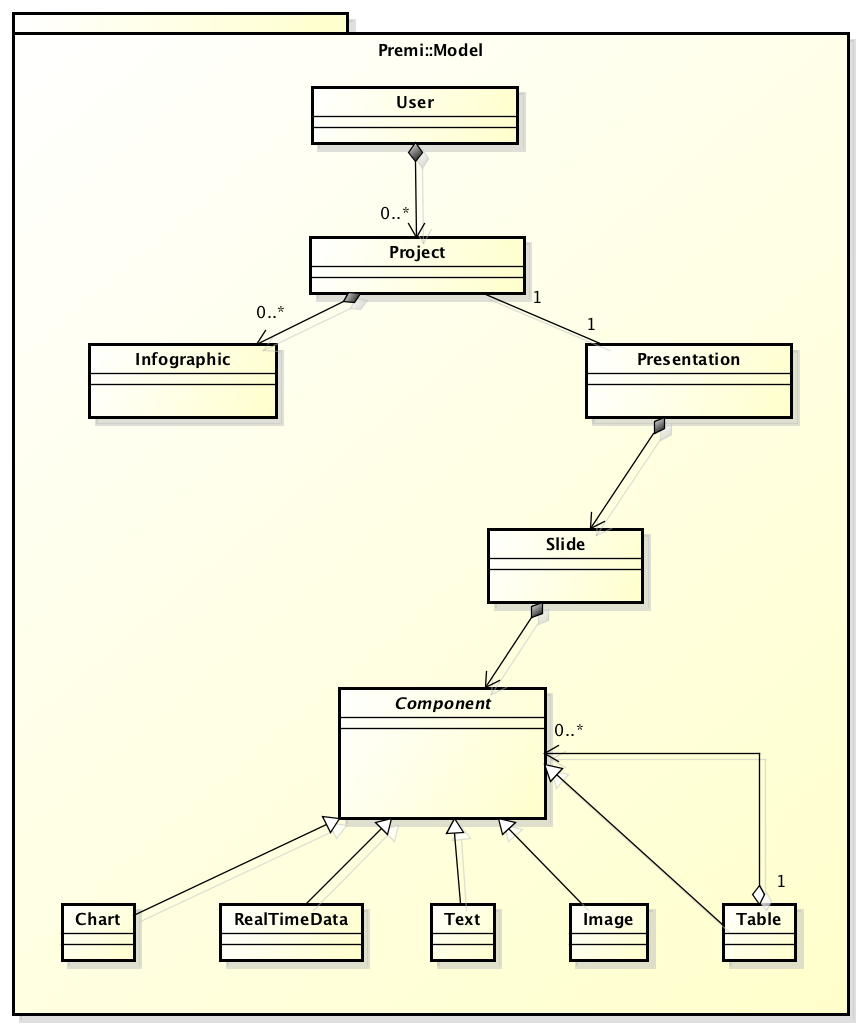
\includegraphics[width=0.7\linewidth]{img/premi_model}
		\caption[Premi::Model]{Premi::Model}
		\label{fig:premi_model}
	\end{figure}
	
Il package gestisce lo scambio di informazioni tra una sorgente dati e l'interfaccia utente, attraverso i controller. Per ottenere informazioni si comunica con il model. Tutti i model comunicano tra di loro andando a costruire una serie di relazioni che rendono più semplice e veloce il recupero dei dati da parte del controller. Laravel utilizza un proprio ORM(Object Relational Mapping) chiamato Eloquent. Tutti i model estendono Eloquent che permette l'integrazione del database con il tipo di programmazione utilizzata.

	\newpage
\subsubsection{User}

	\begin{figure}[h]
		\centering
		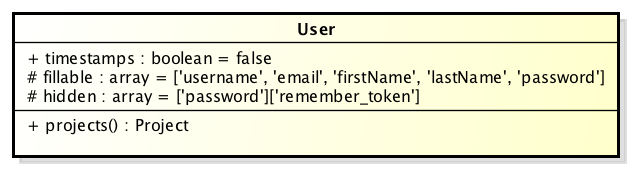
\includegraphics[width=0.7\linewidth]{img/User}
		\caption[Diagramma della classe User]{Diagramma della classe User}
		\label{fig:User}
	\end{figure}

	\subsubsection*{Descrizione}
	Il model User permette di gestire la collection users del database. Eloquent presume che il nome della classe sia il singolare del nome della collection nel database, quindi collega USer alla collection users.
	\subsubsection*{Utilizzo}
	Il model gestisce la collection users del database.
	\subsubsection*{Attributi}
	\begin{itemize}
		\item \textbf{+ timestamps : boolean = false :}\\
		Di default Eloquent automatizza l'inserimento del timestamp relativo all'inserimento e aggiornamento di un campo. Se alla variabile viene assegnato il valore le informazioni dell'inserimento e del aggiornamento non verranno aggiunto alla collection.
		\item \textbf{\# fillable : array = ['username', 'email', 'firstName', 'lastName', 'password']:}\\
		Quando si crea un model, si deve passare una serie di attributi al costruttore del model stesso. Questi attributi vengono assegnati al model tramite \textbf{mass assignment}. La propietà \textit{fillable} serve a specificare quali attributi devono essere assegnabili tramite il mass-assignment.
		\item \textbf{\# hidden : array = ['password', 'remember\_token''] : }\\
		La proprietà hidden si aggiunge quando si vuole limitare gli attributi che sono inclusi nel JSON.
	\end{itemize}
	\subsubsection*{Metodi}
	\begin{itemize}
		\item \textbf{+ projects() : Project}\\
		Abbiamo utilizzato la relazione embedsMany per riuscire ad incorporare il model projects all'interno dell'oggetto principale User. Il metodo ritorna Project su cui verrà chiamato il metodo save() nel caso in cui si voglia aggiornare il modello.
	\end{itemize}
	
\newpage
\subsubsection{Project}

%figura

	\subsubsection*{Descrizione}
	Il model Project rappresenta un progetto creato da un utente. Contiene la presentazio e una o
più infografiche create da esso o nessuna.

	\subsubsection*{Utilizzo}
	Viene utilizzato alla creazione o caricamento di un progetto.
	
	\subsubsection*{Attributi}
	\begin{itemize}
		\item \textbf{+ timestamps : boolean = false :}\\
		Di default Eloquent automatizza l'inserimento del timestamp relativo all'inserimento e aggiornamento di un campo. Se alla variabile viene assegnato il valore le informazioni dell'inserimento e del aggiornamento non verranno aggiunto alla collection.
		\item \textbf{\# fillable : array = [’name’]:}\\
		Quando si crea un model, si deve passare una serie di attributi al costruttore del model stesso. Questi attributi vengono assegnati al model tramite \textbf{mass assignment}. La propietà \textit{fillable} serve a specificare quali attributi devono essere assegnabili tramite il mass-assignment.
		\item \textbf{\# hiddem : array = ['password', 'remember\_token''] : }\\
		La proprietà hidden si aggiunge quando si vuole limitare gli attributi che sono inclusi nel JSON.
	\end{itemize}
	
	\subsubsection*{Metodi}
	\begin{itemize}
		\item \textbf{+ presentation() : Presentation}\\
		Abbiamo utilizzato la relazione embedsOne per riuscire ad incorporare il model Presentation all’interno dell’oggetto principale Project. Il metodo ritorna Presentation su cui verrà chiamato il metodo save() nel caso in cui si voglia aggiornare il modello.
		\item \textbf{+ infographics() : Infographics}\\
		Abbiamo utilizzato la relazione embedsMany per riuscire ad incorporare il model Infographic all’interno dell’oggetto principale Project. Il metodo ritorna Infographic su cui verrà chiamato il metodo save() nel caso in cui si voglia aggiornare il modello.
	\end{itemize}

\newpage
\subsubsection{Infographic}

%figure

	\subsubsection*{Descrizione}
	Questa classe rappresenta un’infografica di un progetto, ovvero una rappresentazione visuale della presentazione per mostrare in maniera semplice e veloce le informazioni.
	
	\subsubsection*{Utilizzo}
Viene utilizzata alla creazione di un’infografica di una presentazione.

\subsubsection*{Attributi}
	\begin{itemize}
		\item \textbf{+ timestamps : boolean = false :}\\
		Di default Eloquent automatizza l'inserimento del timestamp relativo all'inserimento e aggiornamento di un campo. Se alla variabile viene assegnato il valore le informazioni dell'inserimento e del aggiornamento non verranno aggiunto alla collection.
		\item \textbf{\# fillable : array = [’name’, ’path’]:}\\
		Quando si crea un model, si deve passare una serie di attributi al costruttore del model stesso. Questi attributi vengono assegnati al model tramite \textbf{mass assignment}. La propietà \textit{fillable} serve a specificare quali attributi devono essere assegnabili tramite il mass-assignment.
	\end{itemize}


\newpage
\subsubsection{Presentation}

	%figura

	\subsubsection*{Descrizione}
	Questa classe descrive la presentazione di un progetto. Contiene tutte le slide che servono a comporre la presentazione.

	\subsubsection*{Utilizzo}
	Viene utilizzato alla creazione o caricamento di una presentazione.
	
	\subsubsection*{Attributi}
	\begin{itemize}
		\item \textbf{+ timestamps : boolean = false :}\\
		Di default Eloquent automatizza l'inserimento del timestamp relativo all'inserimento e aggiornamento di un campo. Se alla variabile viene assegnato il valore le informazioni dell'inserimento e del aggiornamento non verranno aggiunto alla collection.
		\item \textbf{\# fillable : array = ['title']:}\\
		Quando si crea un model, si deve passare una serie di attributi al costruttore del model stesso. Questi attributi vengono assegnati al model tramite \textbf{mass assignment}. La propietà \textit{fillable} serve a specificare quali attributi devono essere assegnabili tramite il mass-assignment.
	\end{itemize}

	\subsubsection*{Metodi}
	\begin{itemize}
		\item \textbf{+ slides() : Slide}\\
		Abbiamo utilizzato la relazione embedsMany per riuscire ad incorporare il model Slide all’interno dell’oggetto principale Presentation. Il metodo ritorna Slide su cui verrà chiamato il metodo save() nel caso in cui si voglia aggiornare il modello.
	\end{itemize}
\newpage

\subsubsection{Slide}

	%figura

	\subsubsection*{Descrizione}
	Questa classe descrive una singola slide. Contiene tutti i gli oggetti appartenenti alla slide.
	
	\subsubsection*{Utilizzo}
Viene utilizzato alla creazione o caricamento di una slide.

	\subsubsection*{Attributi}
	\begin{itemize}
		\item \textbf{+ timestamps : boolean = false :}\\
		Di default Eloquent automatizza l'inserimento del timestamp relativo all'inserimento e aggiornamento di un campo. Se alla variabile viene assegnato il valore le informazioni dell'inserimento e del aggiornamento non verranno aggiunto alla collection.
		\item \textbf{\# fillable : array = [’xIndex’, ’yIndex']:}\\
		Quando si crea un model, si deve passare una serie di attributi al costruttore del model stesso. Questi attributi vengono assegnati al model tramite \textbf{mass assignment}. La propietà \textit{fillable} serve a specificare quali attributi devono essere assegnabili tramite il mass-assignment.
	\end{itemize}
	\subsubsection*{Metodi}
	\begin{itemize}
		\item \textbf{+ components() : Component}\\
		Abbiamo utilizzato la relazione embedsMany per riuscire ad incorporare il model Component all’interno dell’oggetto principale Slide. Il metodo ritorna Component su cui verrà chiamato il metodo save() nel caso in cui si voglia aggiornare il modello.
	\end{itemize}
\newpage

\subsubsection{Component}

	%figura

	\subsubsection*{Descrizione}
	Questa classe descrive la struttura genera di un componente.
	
	\subsubsection*{Utilizzo}
	Viene utilizzato alla creazione o caricamento di una componente.
	
	\subsubsection*{Attributi}
	\begin{itemize}
		\item \textbf{+ timestamps : boolean = false :}\\
		Di default Eloquent automatizza l'inserimento del timestamp relativo all'inserimento e aggiornamento di un campo. Se alla variabile viene assegnato il valore le informazioni dell'inserimento e del aggiornamento non verranno aggiunto alla collection.
		\item \textbf{\# fillable : array = [’type’, ’originX’, ’OriginY’, ’left’, ’top’, ’width’, ’height’, ’fill’, ’stroke’, ’strokeWidth’, ’strokeDashArray’, ’strokeLineCap’, ’strokeLine-Join’, ’strokeMiterLimit’, ’scaleX’, ’scaleY’, ’angle’, ’flipX’, ’flipY’, ’opacity’, ’shadow’, ’visible’, ’clipTo’, ’backgroundColor’, ’fillRule’, ’globalCompositeOperation']:}\\
		Quando si crea un model, si deve passare una serie di attributi al costruttore del model stesso. Questi attributi vengono assegnati al model tramite \textbf{mass assignment}. La propietà \textit{fillable} serve a specificare quali attributi devono essere assegnabili tramite il mass-assignment.
	\end{itemize}
	

\newpage
\subsubsection{Chart}

%figura

	\subsubsection*{Descrizione}
	Questa classe rappresenta la struttura di dati necessari per descrivere un grafico all’interno di una slide.
	
	\subsubsection*{Utilizzo}
Viene utilizzato alla creazione o caricamento di un grafico.

	\subsubsection*{Attributi}
	\begin{itemize}
		\item \textbf{+ timestamps : boolean = false :}\\
		Di default Eloquent automatizza l'inserimento del timestamp relativo all'inserimento e aggiornamento di un campo. Se alla variabile viene assegnato il valore le informazioni dell'inserimento e del aggiornamento non verranno aggiunto alla collection.
		\item \textbf{\# fillable : array = [’typeChart’ , ’data’]:}\\
		Quando si crea un model, si deve passare una serie di attributi al costruttore del model stesso. Questi attributi vengono assegnati al model tramite \textbf{mass assignment}. La propietà \textit{fillable} serve a specificare quali attributi devono essere assegnabili tramite il mass-assignment.
		
	\end{itemize}
	

\newpage
\subsubsection{RealTimeData}

%figura

	\subsubsection*{Descrizione}
	Questa classe rappresenta la struttura di dati necessari per descrivere RealTimeData (dato in tempo reale) all’interno di una slide.
	
	\subsubsection*{Utilizzo}
	Viene utilizzato alla creazione o caricamento di un RealTimeData.
	
	\subsubsection*{Attributi}
	\begin{itemize}
		\item \textbf{+ timestamps : boolean = false :}\\
		Di default Eloquent automatizza l'inserimento del timestamp relativo all'inserimento e aggiornamento di un campo. Se alla variabile viene assegnato il valore le informazioni dell'inserimento e del aggiornamento non verranno aggiunto alla collection.
		\item \textbf{\# fillable : array = ['pathParser’, ’pathFallback’, ’pathHandlerJs']:}\\
		Quando si crea un model, si deve passare una serie di attributi al costruttore del model stesso. Questi attributi vengono assegnati al model tramite \textbf{mass assignment}. La propietà \textit{fillable} serve a specificare quali attributi devono essere assegnabili tramite il mass-assignment.
		
	\end{itemize}
	
	
\newpage
\subsubsection{Text}

	%figura

	\subsubsection*{Descrizione}
	Questa classe rappresenta la struttura di dati di un campo di testo di una slide.
	
	\subsubsection*{Utilizzo}
	Viene utilizzato alla creazione o caricamento di un campo di testo.
	
	\subsubsection*{Attributi}
	\begin{itemize}
		\item \textbf{+ timestamps : boolean = false :}\\
		Di default Eloquent automatizza l'inserimento del timestamp relativo all'inserimento e aggiornamento di un campo. Se alla variabile viene assegnato il valore le informazioni dell'inserimento e del aggiornamento non verranno aggiunto alla collection.
		\item \textbf{\# fillable : array = [’text’, ’fontSize’, ’fontWeight’, ’fontFamily’, ’fontStyle’, ’lineHeight’, ’textDecoration’, ’textAlign’, ’textBackgroundColor']:}\\
		Quando si crea un model, si deve passare una serie di attributi al costruttore del model stesso. Questi attributi vengono assegnati al model tramite \textbf{mass assignment}. La propietà \textit{fillable} serve a specificare quali attributi devono essere assegnabili tramite il mass-assignment.

	\end{itemize}

\newpage
\subsubsection{Image}

	%figura

	\subsubsection*{Descrizione}
	La classe Image rappresenta la struttura dei dati necessari per rapresentare un’immagine all’interno di una slide.
	
	\subsubsection*{Utilizzo}
	Utilizzata quando viene inserita un’immagine per tenerne traccia.
	
	\subsubsection*{Attributi}
	\begin{itemize}
		\item \textbf{+ timestamps : boolean = false :}\\
		Di default Eloquent automatizza l'inserimento del timestamp relativo all'inserimento e aggiornamento di un campo. Se alla variabile viene assegnato il valore le informazioni dell'inserimento e del aggiornamento non verranno aggiunto alla collection.
		\item \textbf{\# fillable : array = [’src’, ’filters’, ’crossOrigin’, ’alignX’, ’alignY’,’meetOrSlice’, ’background’]:}\\
		Quando si crea un model, si deve passare una serie di attributi al costruttore del model stesso. Questi attributi vengono assegnati al model tramite \textbf{mass assignment}. La propietà \textit{fillable} serve a specificare quali attributi devono essere assegnabili tramite il mass-assignment.

	\end{itemize}

\newpage
\subsubsection{Table}

	%figura

	\subsubsection*{Descrizione}
	Questa classe rappresenta la struttura di dati di una tabella di una slide.
	
	\subsubsection*{Utilizzo}
	Viene utilizzato alla creazione o caricamento di una tabella.
	
	\subsubsection*{Attributi}
	\begin{itemize}
		\item \textbf{+ timestamps : boolean = false :}\\
		Di default Eloquent automatizza l'inserimento del timestamp relativo all'inserimento e aggiornamento di un campo. Se alla variabile viene assegnato il valore le informazioni dell'inserimento e del aggiornamento non verranno aggiunto alla collection.
		\item \textbf{\# fillable : array = [’row’, ’column’, ’title’, ’cellData’]:}\\
		Quando si crea un model, si deve passare una serie di attributi al costruttore del model stesso. Questi attributi vengono assegnati al model tramite \textbf{mass assignment}. La propietà \textit{fillable} serve a specificare quali attributi devono essere assegnabili tramite il mass-assignment.

	\end{itemize}
\newpage
%\input {sections/nomesezione}
%\newpage

% ...

%\printglossaries

\end{document}
